\documentclass[12pt, a4paper]{article}

% Nödvändiga paket för matematik och grafik
\usepackage{amsmath}
\usepackage{tikz}
\usepackage{xcolor}
\usepackage[margin=1in]{geometry}

% Sidhuvud
\title{\textbf{The GERC Mechanism and the Non-Singular Bounce}}
\author{Advanced Research Center for Quantum Geometry}
\date{}

\begin{document}

\maketitle

\section*{Analytical Formulation: The GERC Regulatory Response}

In classical General Relativity, gravitational collapse drives the metric curvature toward an unbounded limit as the radius $r$ approaches zero. In the SAGD framework, the Gauge-Equivariant Ricci Controller (GERC) remains dormant in the weak-curvature regime but introduces a rapid regulatory response as compression approaches the phase-space regulatory scale $r_{reg}$.

We can define a simplified effective curvature model to simulate this divergence versus regulation:
\begin{equation}
    \mathcal{K}_{classical}(r) = \frac{G M}{r^3}
\end{equation}

To model the SAGD active grid response, we introduce a geometric suppression factor that redirects the metric compression into torsional channels once $r \sim r_{reg}$:
\begin{equation}
    \mathcal{K}_{SAGD}(r) = \frac{G M}{r^3} \left[ 1 - \exp\left(-\left(\frac{r}{r_{reg}}\right)^4\right) \right]
\end{equation}

As $r \to 0$, the exponential term expands to $1 - (r/r_{reg})^4$, causing the metric curvature to peak and then smoothly decay to zero at the exact center, representing the formation of the finite torsional core.

\vspace{1cm}

% TikZ-figur för Channel Shift
\begin{figure}[h!]
    \centering
    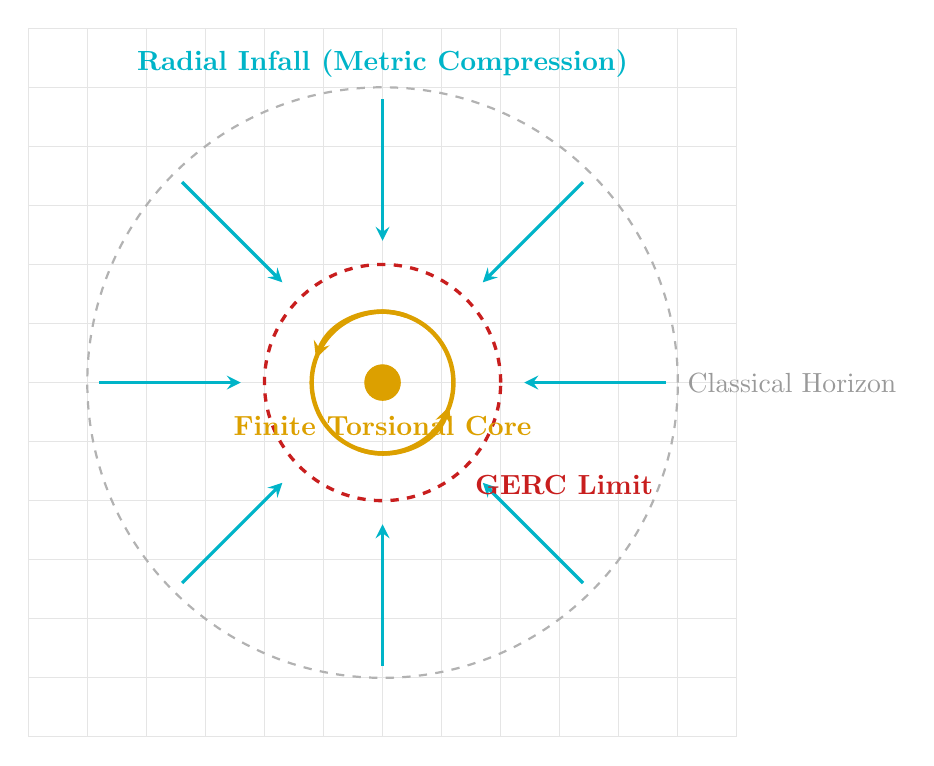
\begin{tikzpicture}[>=stealth, scale=1.5]

        % Define colors matching the repository theme
        \definecolor{sagdred}{RGB}{200, 30, 30}
        \definecolor{sagdcyan}{RGB}{0, 180, 200}
        \definecolor{sagdyellow}{RGB}{220, 160, 0}

        % Background grid to represent the active manifold
        \draw[step=0.5, gray!20, thin] (-3,-3) grid (3,3);

        % Outer classical metric limit
        \draw[thick, dashed, gray!60] (0,0) circle (2.5);
        \node[gray!80, right] at (2.5, 0) {Classical Horizon};

        % Infalling metric compression (Radial Arrows)
        \foreach \angle in {0, 45, 90, 135, 180, 225, 270, 315} {
            \draw[->, very thick, sagdcyan] (\angle:2.4) -- (\angle:1.2);
        }
        \node[sagdcyan, above] at (0, 2.5) {\textbf{Radial Infall (Metric Compression)}};

        % The Regulatory Phase-Space Boundary
        \draw[very thick, sagdred, dashed] (0,0) circle (1.0);
        \node[sagdred, below right] at (0.7, -0.7) {\textbf{GERC Limit}};

        % Torsional Core (Circulation Arrows)
        \draw[->, ultra thick, sagdyellow] (0,0) +(70:0.6) arc (70:340:0.6);
        \draw[->, ultra thick, sagdyellow] (0,0) +(250:0.6) arc (250:520:0.6);
        
        % Core center
        \filldraw[sagdyellow] (0,0) circle (0.15);
        \node[sagdyellow, below] at (0, -0.2) {\textbf{Finite Torsional Core}};

    \end{tikzpicture}
    \caption{The Metric-to-Torsion Channel Shift.}
    \label{fig:channel_shift}
\end{figure}

\end{document}
